\apendice{Plan de Proyecto Software}

\section{Introducción}

En este apartado se presenta la planificación temporal del proyecto empleando la metodología SCRUM, así como la viabilidad del proyecto desde el punto de vista legal y económico.

\section{Planificación temporal}

Como se ha indicado en el apartado anterior, para el desarrollo del proyecto se siguió la metodología \textit{SCRUM}, adaptándola a las necesidades y al tiempo disponible. Las características a destacar de esta metodología son las siguientes:

\begin{itemize}
    \item Desarrollo iterativo e incremental que permite adaptarse a cambios inesperados en los requerimientos o herramientas empleadas.
    \item El proyecto se subdivide en múltiples tareas, que se abordan a lo largo de varias iteraciones denominadas \textit{sprints}.
    \item Todos los \textit{sprints} tienen una duración prefijada, en este caso de 2 semanas.
    \item Todo \textit{sprint} se inicia o finaliza con una reunión con el tutor del proyecto.
\end{itemize}

\subsection{Sprint 0}
Durante el \textit{sprint 0} se abordaron las tareas requeridas para la inicialización del proyecto, así como la evaluación y la toma de decisión de las distintas herramientas que se pretendían utilizar durante la posterior implementación.

\begin{table}[H]
    \centering
    \begin{tabular}{l}
    \hline
    \textbf{Tareas} \\ \hline
    Creación del repositorio del proyecto \\
    Creación del entorno de trabajo \\
    Evaluación de la forma de extraer hashtags de Instagram \\
    Evaluación de los distintos \textit{crawlers} y herramientas a utilizar \\
    Registro y experimentación con las herramientas de Google Cloud \\ \hline
    \end{tabular}
    \caption{Tareas del \textit{sprint 0}}
    \label{tab:tasks_sprint0}
\end{table}

\subsection{Sprint 1}
Durante el \textit{sprint 1} se abordaron las tareas relacionadas con la automatización de la descarga de publicaciones de Instagram y se inició el desarrollo de la memoria.

\begin{table}[H]
    \centering
    \begin{tabular}{l}
    \hline
    \textbf{Tareas} \\ \hline
    Creación de la máquina virtual \\
    Implementación de la descarga de publicaciones mediante Instalooter \\
    Subida de publicaciones a un \textit{blob} de Google Cloud \\
    Pruebas de reconocimiento facial con Cloud Vision \\
    Documentación sobre la metodología PRISMA para map-review \\
    Inicio de la memoria en Overleaf \\ \hline
    \end{tabular}
    \caption{Tareas del \textit{sprint 1}}
    \label{tab:tasks_sprint1}
\end{table}

\subsection{Sprint 2}
Durante el \textit{sprint 2} se evaluaron las alternativas a Cloud Vision tras comprobar que no se podía extraer la edad ni el género. También se redactó la parte de trabajos relacionados o el estado del arte de la memoria.

\begin{table}[H]
    \centering
    \begin{tabular}{l}
    \hline
    \textbf{Tareas} \\ \hline
    Evaluación de las alternativas a Cloud Vision y Google Cloud \\
    Pruebas con Microsoft Azure \\
    Pruebas con Amazon Web Services \\
    Elección de los artículos relacionados \\
    Redacción del apartado de Trabajo relacionados \\ \hline
    \end{tabular}
    \caption{Tareas del \textit{sprint 2}}
    \label{tab:tasks_sprint2}
\end{table}

\subsection{Sprint 3}
Durante el \textit{sprint 3} se decidió emplear Amazon Web Services tras comprobar que era la mejor alternativa. Se llevaron a cabo los cambios en los scripts y se implementó la descarga de datos de reconocimiento facial.

\begin{table}[H]
    \centering
    \begin{tabular}{l}
    \hline
    \textbf{Tareas} \\ \hline
    Adaptación de los scripts para usar los servicios de Amazon \\
    Implementación de la descarga de datos de Rekognition \\
    Evaluación de las posibles bases de datos a utilizar \\
    Evaluación de las posibles visualizaciones a implementar \\ \hline
    \end{tabular}
    \caption{Tareas del \textit{sprint 3}}
    \label{tab:tasks_sprint3}
\end{table}

\subsection{Sprint 4}

Durante el \textit{sprint 4} se diseñó e implementó la base de datos en DynamoDB. También se tuvo que llevar a cabo una corrección en Instalooter después de que dejara de funcionar.

\begin{table}[H]
    \centering
    \begin{tabular}{l}
    \hline
    \textbf{Tareas} \\ \hline
    Diseño e implementación de la base de datos \\
    Implementación de los scripts de subida de datos a DynamoDB \\
    Hotfix de Instalooter \\
    Evaluación de los posibles dashboards a utilizar \\ \hline
    \end{tabular}
    \caption{Tareas del \textit{sprint 4}}
    \label{tab:tasks_sprint4}
\end{table}

\subsection{Sprint 5}

Durante el \textit{sprint 5} se tomó la decisión de implementar un cuadro de mandos con Grafana, para ello se iniciaron las pruebas para crear un conector con DynamoDB, también se finalizó el script para poblar la base de datos.

\begin{table}[H]
    \centering
    \begin{tabular}{l}
    \hline
    \textbf{Tareas} \\ \hline
    Creación del script final de descarga y subida de datos a DynamoDB \\
    Llenado de la base datos \\
    Pruebas con Grafana \\
    Desarrollo de un servidor local para conectar Grafana con DynamoDB \\ \hline
    \end{tabular}
    \caption{Tareas del \textit{sprint 5}}
    \label{tab:tasks_sprint5}
\end{table}

\subsection{Sprint 6}

Durante el \textit{sprint 6} se finalizó el conector de Grafana con DynamoDB, se implementó el cuadro de mandos final y se continuó con la redacción de la memoria.

\begin{table}[H]
    \centering
    \begin{tabular}{l}
    \hline
    \textbf{Tareas} \\ \hline
    Portado del conector de Grafana a AWS Lambda y Amazon API Gateway \\
    Diseño e implementación final del Dashboard \\
    Redacción del apartado de Objetivos del proyecto \\
    Redacción del apartado de Conceptos teóricos \\
    Redacción del apartado de Técnicas y herramientas \\ \hline
    \end{tabular}
    \caption{Tareas del \textit{sprint 6}}
    \label{tab:tasks_sprint6}
\end{table}

\subsection{Sprint 7}

Durante el \textit{sprint 7} se finalizó la memoria y se reorganizó el repositorio de cara a la entrega final.

\begin{table}[H]
    \centering
    \begin{tabular}{l}
    \hline
    \textbf{Tareas} \\ \hline
    Redacción del apartado de Introducción \\
    Redacción del apartado de Aspectos relevantes del desarrollo del proyecto \\
    Redacción del apartado de Conclusiones y líneas de trabajo futuras \\
    Redacción de los apéndices \\ \hline
    \end{tabular}
    \caption{Tareas del \textit{sprint 7}}
    \label{tab:tasks_sprint7}
\end{table}

\section{Estudio de viabilidad}

\subsection{Viabilidad económica}

En este apartado se describe el coste estimado del proyecto.

\subsubsection{Costes de personal}

Mediante el ``XVII Convenio colectivo estatal de empresas de consultoría y estudios'' publicado en el BOE Núm. 57 el 6 de marzo de 2018, podemos obtener los costes del personal. En este proyecto se ha empleado a un Analista Programador durante 4 meses. De acuerdo al anterior documento se puede concluir que el salario mensual a tiempo completo es de 1.916,15€. Como la dedicación ha sido parcial, el sueldo es de 958,07€.

\begin{table}[H]
    \centering
    \begin{tabular}{p{0.17\textwidth}lll|c}
    \hline
    \textbf{Tarea} & \textbf{Perfil} & \textbf{Salario mensual} & \textbf{Meses} & \textbf{Total} \\ \hline
    Desarrollo del proyecto & Analista Programador & 958,07€ & 4 & 3.832,29€ \\ \hline
    \end{tabular}
    \caption{Costes de personal}
    \label{tab:coste_personal}
\end{table}

\subsubsection{Costes de Hardware}

Para el desarrollo del proyecto el único hardware necesario ha sido un \textbf{ordenador personal}, cuyo coste es de 1.139,86€.

\subsubsection{Costes de uso de Amazon Web Services}

Como se ha comentado con anterioridad, en el desarrollo del proyecto no se ha incurrido en ningún coste respecto al uso de Amazon Web Services puesto que se ha empleado su capa gratuita. Pero algunos de los servicios de esta capa gratuita están limitados a tan solo los 12 primeros meses. Es por ello que se ha decidido calcular cual sería el coste mensual del uso de esta plataforma bajo las mismas condiciones que las que se han empleado a lo largo del proyecto. Para ello se ha empleado la \href{https://calculator.aws/#/}{calculadora de coste} de AWS, empleando como región \texttt{eu-west-1} (Irlanda):

\begin{itemize}
    \item \textbf{Amazon EC2}: Empleando una máquina virtual \texttt{t2.micro} con Linux con 30GB de almacenamiento SSD, el coste por hora está a 0,0126 USD. En la capa gratuita, se permite usar hasta 750 horas al mes que son más o menos las que se llegaron a utilizar. Por ello en total el coste calculado al mes es de 9,80 USD.
    \item \textbf{Amazon S3}: Los primeros 50 TB de almacenamiento al mes tienen un coste de 0,023 USD por GB, y en la capa gratuita se permite usar hasta 5GB. Por otro lado, 1000 solicitudes de operaciones PUT cuestan 0,005 USD, y como se ha comentado anteriormente, se usaron las 2000 operaciones de este tipo que se permiten en la capa gratuita. Además, 1000 solicitudes GET son 0,0004 USD, y en la capa gratuita se permite hasta 20000. Por lo tanto, el coste final es de 0,13 USD al mes.
    \item \textbf{Amazon Rekognition}: El coste del primer millón de imágenes está actualmente a 0,001 USD por imagen. Como se han analizado 2000 imágenes al mes el coste estimado es de 2.00 USD.
    \item \textbf{Amazon DynamoDB}: Se tiene 25 GBs gratuitos para siempre, y esto por ahora ha sido más que suficiente, por lo que no habría costes por el almacenamiento y las consultas en la base de datos.
    \item \textbf{AWS Lambda}: Se tiene un millón de operaciones al mes (3,2 millones de segundos) gratuitas para siempre. Esto ha sido más que suficiente durante las pruebas llevadas cabo, con lo que no habría costes por las consultas llevadas a cabo por el cuadro de mandos.
    \item \textbf{Amazon API Gateway}: Las primeras 333 millones de peticiones API de REST tienen un coste 3,50 USD por millón. Como en la capa gratuita se permite hasta un millón, el coste sería de 3,50 USD al mes.
\end{itemize}

\begin{figure}[H]
    \centering
    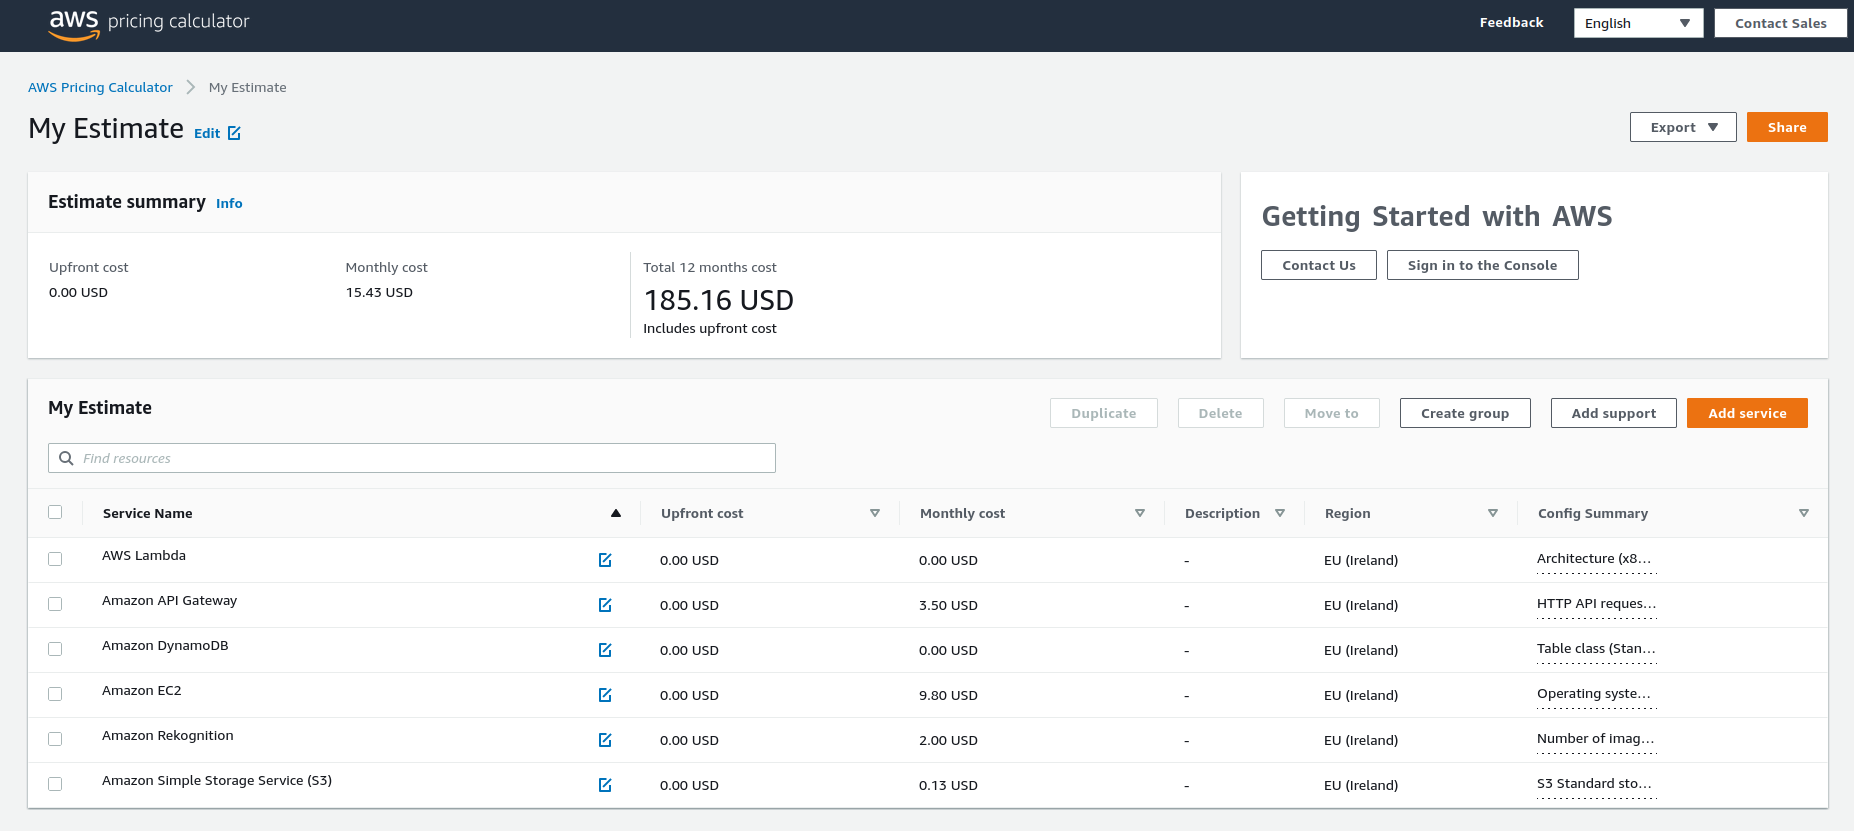
\includegraphics[width=1.0\textwidth]{memoria/img/coste_aws.png}
    \caption{Cálculo de coste con la calculadora de AWS}
    \label{fig:coste_aws}
\end{figure}

Por lo tanto, mensualmente el coste estimado sería de 15,43 USD por usar los servicios de AWS. Como en la actualidad el tipo de cambio es de 1,00 USD = 1,00 EUR, el coste final sería el siguiente:

\begin{table}[H]
    \centering
    \begin{tabular}{cc|c}
    \hline
    \textbf{Coste mensual} & \textbf{Meses} & \textbf{Total} \\ \hline
    15,43€ & 4 & 61,72€ \\ \hline
    \end{tabular}
    \caption{Costes de uso de AWS}
    \label{tab:coste_aws}
\end{table}

\subsubsection{Beneficio industrial}

Según el artículo 101.2 de la Ley 9/2017 de Contratos del Sector Público (LCSP) el beneficio industrial se calcula como el 6\% del coste total del proyecto sin aplicar el IVA. Por lo tanto el beneficio industrial generado es el siguiente:

\begin{table}[H]
    \centering
    \begin{tabular}{ll}
    \hline
    \textbf{Concepto}           & \textbf{Valor (€)} \\ \hline
    Coste de personal           & 3.832,29€      \\
    Costes de hardware          & 1.139,86€ \\
    Costes de AWS               & 61,72€ \\ \hline
    Subtotal                    & 5.033,87€ \\ \hline
    Beneficio industrial (6\%)  & 302,03€ \\ \hline
    \end{tabular}
    \caption{Beneficio industrial}
    \label{tab:beneficio_industrial}
\end{table}

\subsubsection{Coste total}

El coste total tras contar todos los subapartados anteriores se puede ver en la siguiente tabla:

\begin{table}[H]
    \centering
    \begin{tabular}{ll}
    \hline
    \textbf{Concepto}           & \textbf{Valor (€)} \\ \hline
    Coste de personal           & 3.832,29€      \\
    Costes de hardware          & 1.139,86€ \\
    Costes de AWS               & 61,72€ \\ \hline
    Beneficio industrial (6\%)  & 302,03€ \\ \hline
    Subtotal                    & 5.335,90€ \\
    IVA (21\%)                  & 1.120,54€ \\ \hline
    Total                       & 6.456,44€ \\ \hline
    \end{tabular}
    \caption{Coste total}
    \label{tab:coste_total}
\end{table}

\subsection{Viabilidad legal}

En esta sección se muestran las licencias empleadas por las distintas librerías y herramientas utilizadas a lo largo del proyecto, y se describe la licencia finalmente empleada para la publicación del mismo.

Los herramientas empleadas durante el desarrollo del proyecto emplean las siguientes licencias:

\begin{table}[H]
    \centering
    \begin{tabular}{ll}
    \hline
    \textbf{Herramienta} & \textbf{Licencia} \\ \hline
    boto3 & Apache License 2.0 \\
    fs-s3fs & MIT \\
    Instalooter & GPL v3.0 \\
    Grafana & AGPL v3.0 \\
    JSON API Grafana Datasource & MIT \\ \hline
    \end{tabular}
    \caption{Licencias de las herramientas utilizadas}
    \label{tab:licencias}
\end{table}

Por lo tanto, se ha decidido que el proyecto emplee la licencia GPL v3.0, ya que es compatible con todas las anteriores licencias. Entre otras características, esta licencia permite el uso comercial y privado, la modificación y redistribución del código, y a la vez protege ante problemas de garantía, pero al mismo tiempo obliga a que cualquier herramienta que haga uso del proyecto tenga que ser liberada con la misma licencia.
